Other data catalogs in the industry, such as Google's Dataplex~\cite{GoogleDataplex}, allow the user to manually set tags
on dataframes, as a means of categorization and search terminology.
But what if the system could be capable of suggesting possible tags for newly inserted dataframes based on the collection
of previously introduced datasets?
This is the second possible use case of our data matching tool.
It is applicable in situations where we have a large, diverse system, with clearly defined categories of datasets (such as
financial, political, medical, etc.) and we want to determine the most accurate category (or set of categories) of a new entry
without diving into the data and analysing rows by hand.

So far, we have come up with algorithms that match columns.
Tags, on the other hand, are defined on entire dataframes, not individual columns.
To solve this problem, we will be matching every column in our subject dataframe to every column in every other dataframe
in the catalog.
We will add the resulting percentage to a score of each tag of the dataframe that the matched column belongs to.
At the end, we normalize the tags scores with the same normalization formula we used in the previous use case:

normalized\_value = (1 - (value - min\_value) / (max\_value - min\_value)) * 100

This will give us a ``confidence percentage''.
We sort the tags descending by this value and present the best results.

The matching process is much more expensive than the identification of the best column match in just one dataframe, because
this time we are accessing the entire catalog.
We should only use fast algorithms, that make use of the metadata, without accessing the dataframe rows.
In our tests, we have used the following:

\begin{itemize}
    \item Levenshtein distance between the column names
    \item matching data types
    \item similarity of the continuity percentages
    \item similarity of the numerical percentages
    \item number of identical values (we only use this algorithm for a small set of dataframes)
\end{itemize}

There are multiple ways that this matching algorithm can be improved.
If the metadata already contains match results from previous applications of other algorithms, we can use them.
A threshold can also be defined based on previous results of similarity percentages between columns.
For example, if a column has a less than 50\% similarity score to our subject column, it can be skipped.
Similarly, if the best column match in a dataframe has a less than 50\% similarity score to our subject column, the entire
dataframe can be skipped, showing that our previous use case can be used to optimize the current one.
This threshold can be adjusted based on accumulated experience.

Then there is the discussion of which similarity percentages between columns should be counted towards the score of a tag.
If we just sum all of them, then we are biased towards dataframes with many columns, as they will weigh more in the final
result.
To avoid this, we can instead use the average similarity percentage of all columns in a dataframe.
However, tests have shown that using this approach does not significantly alter the final ordering of the best tags, nor
their confidence scores.

Below we will present some practical results obtained by running this algorithm on some subject real world dataframes fetched
from Kaggle~~~~\cite{kaggleHealthAnimalBites,kaggleBigmacPrices,kaggleAllDiets,kaggleRamenRatings}, using a small (20 or less)
set of tagged dataframes as the basis of the tag suggestions.

\begin{figure}[h]
    \centering
    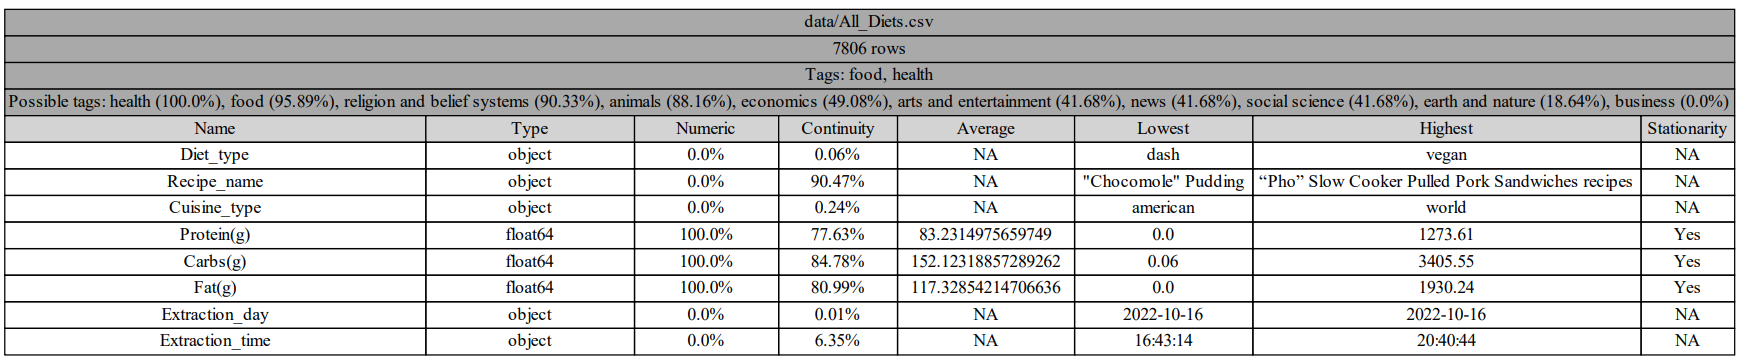
\includegraphics[width=12cm]{figures/tag_suggestions/all_diets_tags}
    \caption{Metadata with tag suggestions for the ``All Diets'' dataframe}
    \label{fig:all_diets_tags}
\end{figure}

\begin{figure}[h]
    \centering
    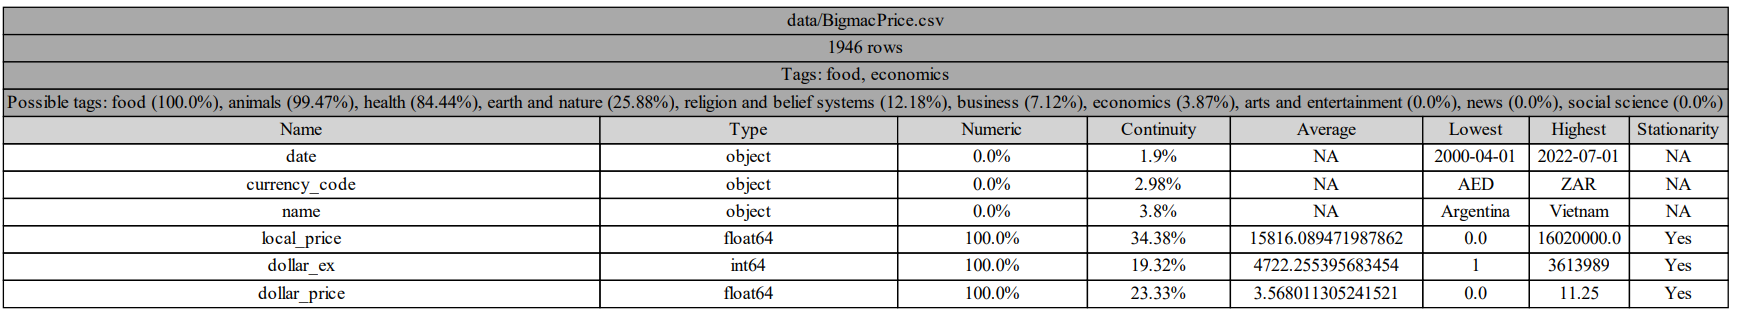
\includegraphics[width=12cm]{figures/tag_suggestions/bigmac_price_tags}
    \caption{Metadata with tag suggestions for the ``Bigmac Prices'' dataframe}
    \label{fig:bigmac_price_tags}
\end{figure}

\begin{figure}[h]
    \centering
    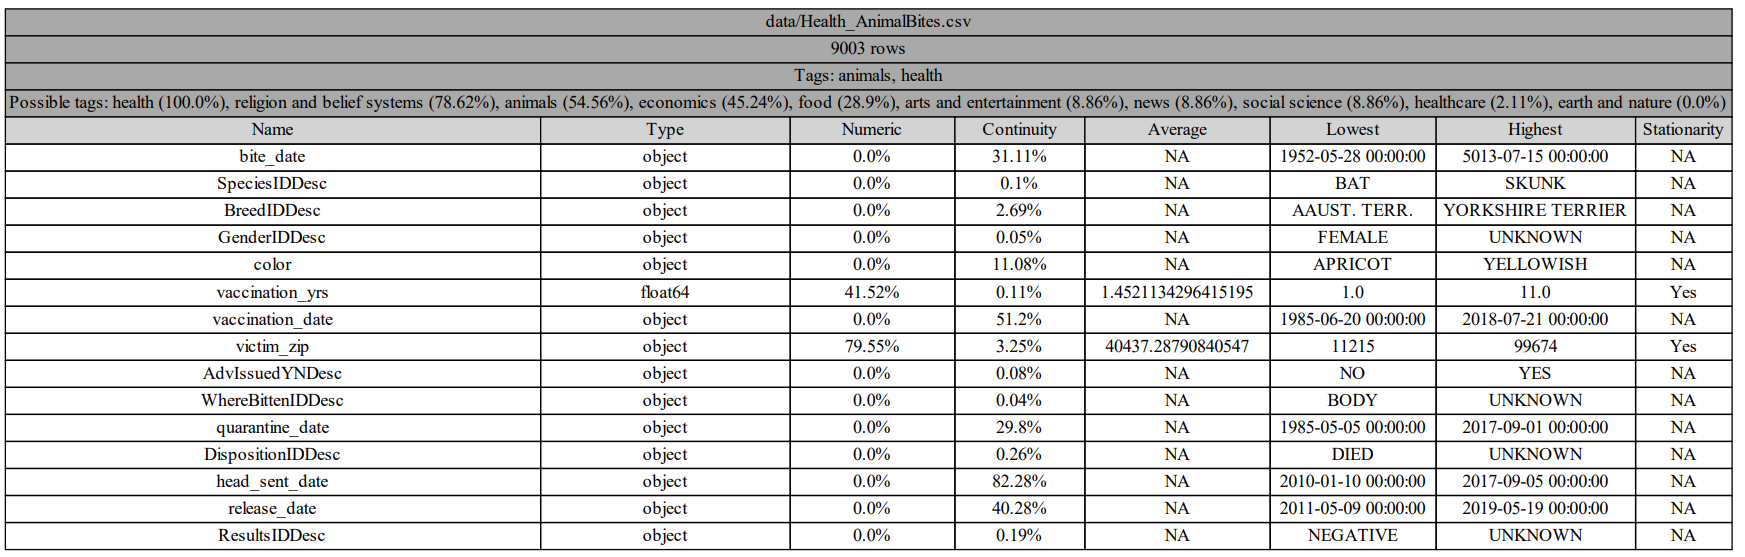
\includegraphics[width=12cm]{figures/tag_suggestions/health_animal_bites_tags}
    \caption{Metadata with tag suggestions for the ``Animal Bites'' dataframe}
    \label{fig:animal_bites_tags}
\end{figure}

\begin{figure}[h]
    \centering
    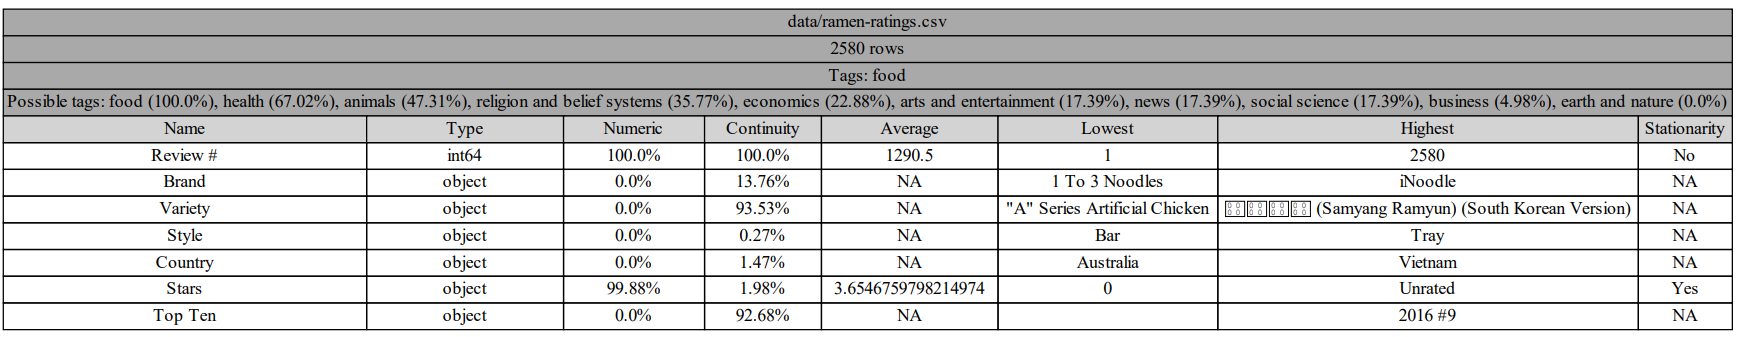
\includegraphics[width=12cm]{figures/tag_suggestions/ramen_ratings_tags}
    \caption{Metadata with tag suggestions for the ``Ramen Ratings'' dataframe}
    \label{fig:ramen_ratings_tags}
\end{figure}

In the resulting metadata, the ``tags'' row is filled with the tags that the dataframe was assigned from its source (Kaggle).
We will use these as verification for our system's results.

Comparing the tags and the suggested tags in each of these results, we can observe that the tool is generally accurate.
For example, for the ``All Diets'' dataframe, our tagging tool suggests, with a 100\% confidence, the \textit{health} tag,
and with a 95.89\% confidence the \textit{food} tag.
The \textit{food} tag is also correctly identified, with a 100\% confidence score, in the ``Bigmac Prices'' and ``Ramen Ratings''
dataframes.
However, our system is far from perfect.
In the ``Animal Bites'' dataframe, the \textit{religion and belief systems} tag is the second-best suggestion, which is incorrect.
The right answer, which in this case would be \textit{animals}, comes after it.
In the ``Bigmac Prices'' dataframe, the \textit{economics} tag is only given a 3.87\% confidence score.
This exposes the primary shortcoming of our system: the higher the frequency of a tag in the data catalog, the more likely
it is it will be suggested for any subject dataframe.

Nonetheless, this flaw can be corrected by the size of the catalog.
The more dataframes we have in our catalog, and the more diverse the tags are, the better the predictions will be.
The tags themselves must also be meaningful for the user and consistent throughout the entire system.
If the user defines the \textit{food} tag as ``a dataframe in which culinary items are mentioned directly'' then that definition
must be considered whenever the decision to assign the tag or not is made.
Otherwise, tags will lose their meanings and suggestions will provide no business value.